\documentclass[Rapport]{subfiles}
\begin{document}

\section{Framtida arbete}

En avgränsning för vårt projekt var att jobba inom ramen för en interpreter. 
Detta av flera anledningar, men främst för att det är lättare att göra prototyper för 
olika regler för optimise. Nu när vi har tagit fram fungerande optimeringssemtantik 
är nästa steg att implementera vårt språk i en kompilator.
Med callstacken istället för substitutionsfunktionen tror vi att implementationen
i en kompilator skulle vara mer realiserbar.


Vårt core språk liknar det som både YHC och GHC arbetar med i sina mellansteg.
Det hade varit ytterst intressant att utöka vårt språk så att vi skulle kunna 
vara backend till något större kompilator, eller runtimesystem?
Vi har alltid haft detta i åtanke och det är delvis därför vi ej har någon 
typechecker.


\NOTE{
Info bild som visar en pipe line för vart vår kompilator finns i kedjan.

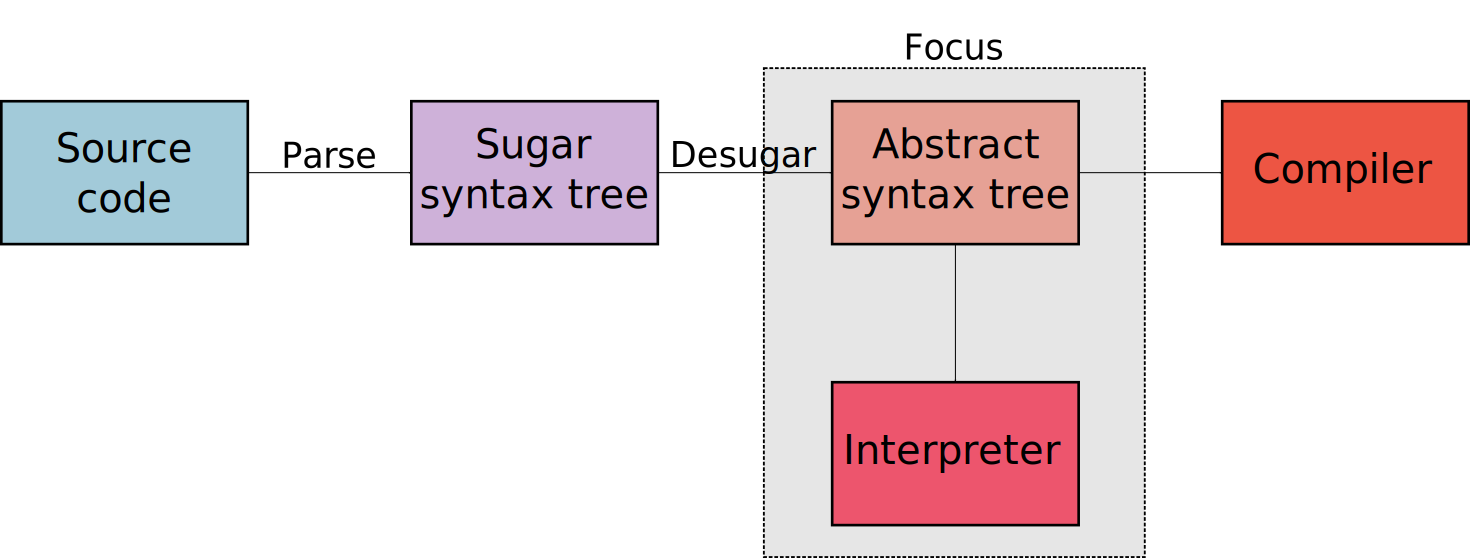
\includegraphics[scale=0.22]{img/pipeline} 
}


En typechecker och stöd för t ex algebric datatypes i ett frontend hade också
varit trevligt då det är väldigt lätt att skriva fel i testprogramen. 


Något annat som föll lite utanför ramen för vårt arbete är att bevisa
korrektheten hos optimisefunktionen, för att se att en optimerad funktion
gör samma sak som dess ooptimerade motsvarighet. Vi har endast använt oss av en testsvit
och andra exempelprogram för att testa optimise. Ett steg för att förvissa sig
om korrektheten skulle vara att göra QuickCheck-egenskaper och generatorer för att se
att en optimerad funktion gör samma sak som en ooptimerad. En annat sätt för att vara säker på att den
gör vad som förväntas vara att formalisera reglerna och bevisa
att de är korrekta, exempelvis med hjälp av en bevisassistent såsom Agda.


\NOTE{
Sharing skulle kunna vara med här (om vi inte får det att fungera).
}

\end{document}
